\chapter{Application examples}
\label{chap:ApplicationExamples}
%
\abstract{In this chapter, three different examples are provided to apply the multi-objective framework and tool presented in this book. First a well known benchmark problem is tackled with the presented methodology and compared with different tuning methods. Then a LiTaO$_3$ Thin Film Deposition Process is used as a prototype for a large dead-time process and tested using a two cost function arrangement. Finally, the MOOTuning software is used to analyze the temperature control in a Continuous Stirred Tank Heater in Section~\ref{sec:CSTH} using two a three cost functions.}
%
\section{High order benchmark plant}
\label{sec:Bechmark}
First the \gls{ennc} method is going to be tested in high order benchmark plant \citep{Astroem2000}. The model of the plant is given by a fourth order transfer function:
\begin{equation}
P(s) = \frac{1}{\prod_{n=0}^{n=3}(0.5^n s+1)}.
\label{eq:benchmarkTF}
\end{equation}

The first step is to obtain a low order model that is able to reflect the main dynamics of the plant. In general, the tuning of \gls{pid} controllers starts with a first or second order model \citep{Alfaro2006}. In this particular case, using a step change as the input signal, the low order model that can be found from this experiment is given by:
%
\begin{equation}
F(s)=\frac{e^{-0.297s}}{(0.9477s+1)(0.6346s+1)},
\label{eq:BenchTFfit}
\end{equation}
%
alternatively, if it is supposed that the ``real'' model of the plant is known, an order reduction procedure, for example, the half-rule method may be used \citep{Skogestad2003}. The comparison between the high order model and the reduced order model in the time domain is presented in %
\begin{figure}[tb]
	\centering
	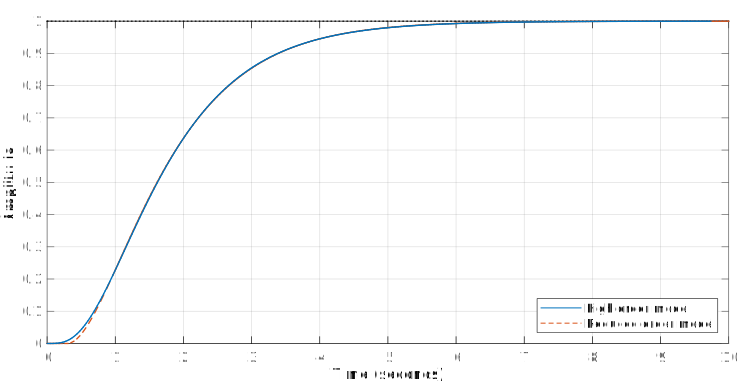
\includegraphics[width=0.9\columnwidth]{Ch7CompRespBench}
	\caption{Comparison between the high and reduced order models.}
	\label{fig:Ch7CompRespBench}
\end{figure}
%
Figure~\ref{fig:Ch7CompRespBench}. As it can be seen, the model represent accurately the dynamics of the original plant and therefore is considered to be a good approximation of the original model.

The next step is to find the Pareto front for this particular plant. The followed methodology was as presented in Chapter~\ref{chap:PIDMOOP}. For this particular case, only $J_{di}$ and $J_r$ where considered as the cost functions with a \gls{2dof} \gls{pid} controller. In Figure~\ref{fig:paretomodelo}, the obtained Pareto front is presented. 
%^
\begin{figure}[tb]%
	\centering
	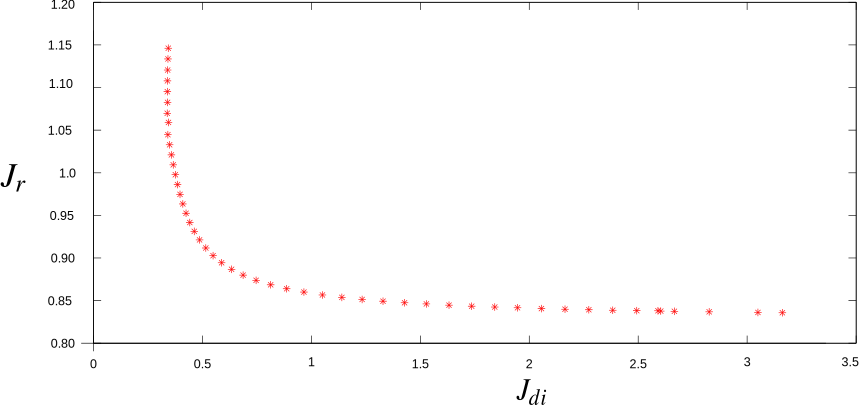
\includegraphics[width=0.9\columnwidth]{paretomodelo}%
	\caption{The Pareto front for the benchmark process.}%
	\label{fig:paretomodelo}%
\end{figure}

The curve has a typical form, with a high slope for low values of $J_{di}$ and an almost flat slope for higher values. This shape has a particular physical meaning: to improve the response of the $J_{di}$ cost function, the $J_{r}$ value has to be augmented (worsening the servo response), however the degradation is not as much as the improvement in the $J_{di}$ function. This is a clear example of one of the many advantages of using a multi-objective framework for controller tuning and the main reason why is the chosen framework in this book, it gives the decision taker more tools to select the more appropriate tuning for the controllers.

In order to compare the response of the optimal controllers, the tuning for the anchor points are presented along the resposes of the ART$_2$ method \citep{Vilanova2011} and the uSORT$_2$ method\citep{Alfaro2012a}, in order to compare the performance of the closed loop response. It is important to clarify that these two tuning are just the extreme points of the Pareto front, thanks to the ENNC method and that there is a practically and infinite amount of possible parameter tuning to select. The obtained parameters are listed in %
%
%parámetros del controlador
\begin{table}[tb]
	\caption{PID controller parameters using two degrees of freedom.}
	\centering
	\begin{tabular}{@{}*{5}{c}@{}}
		\toprule
		Tuning              &$K_c$       &$T_i$      &$T_d$     & $\beta$ 	\\
		\midrule              
		optimum $J_{di}$     &$3.3750$   & $1.0812$  &$0.3095$  &$0.5466$   \\
		optimum $J_{r}$      &$3.0572$   & $8.4419$  &$0.3986$  &$1.2329$   \\
		$ART_2$             &$3.3657$   & $1.7636$  &$0.4884$  &$0.2971$   \\
		$uSORT_2$           &$3.1708$   & $0.8997$  &$0.3945$  &$0.4731$   \\	
		%
		\bottomrule				
	\end{tabular}
	\label{tab:parametroscontrolador}
\end{table}
%
Table~\ref{tab:parametroscontrolador} for reference. It is important to note that in all cases, the Maximum Sensibility was set to be around $M_s = 2.0$ to ensure a minimum level of robustness.

In Figure~\ref{fig:Ch7cambioreferencia}, the closed-loop responses of all the four controllers are presented for the case of a step change in the setpoint. it was found that precisely the controller in the anchor point of the Pareto front that give the minimum value of $J_r$ is in fact the one that give the best result of all the controllers. However, it has to be noticed that both ART$_2$ and uSORT methods are intended for regulator response mainly, and theredore, it was not expected to have a low $J_r$. The obtained values are given in Table~\ref{tab:IAEref} where both the \gls{iae} and \gls{ms} are presented. 

On the other hand, the optimal controllers in the regulator mode are presented in Figure~\ref{fig:cambiodi}. Again, as expected, the controller in the anchor point that has the lowest value of $J_{di}$, is the one with the fastest response. Also, it is clear that the other anchor point (the one with the lowest value of $J_r$) has the worst response for disturbance rejection as it was expected. In table \ref{tab:IAEdi}, the corresponding values of IAE for the curves in Figure~\ref{fig:cambiodi} are presented.

The optimal controller for disturbance rejection is presented in figure \ref{fig:cambiodi}. Again, the tuning given by the ENNC method is the fastest response to reach the desired value. As it can be seen, the ART$_2$ and the uSORT$_{2}$ methods fall between these two optimal responses. However, it does not necessarily means that these methods are optimal because they could be dominated by other controllers that are exactly in the front. Only the tuning found with the ENNC method can be considered to be Pareto optimal using the \gls{iae} as the metric. In Table~\ref{tab:IAEdi}, the IAE values of the responses presented in Figure~\ref{fig:cambiodi} are stated, and again the controller that achieves the lower error value is the one that correspond to the anchor point.
%CAMBIO EN VALOR REFERENCIA
\begin{figure}[tb]%
	\centering
	\includegraphics[width=\columnwidth]{Ch7cambioreferencia}%
	\caption{Optimal response of the control system $J_r$}%
	\label{fig:Ch7cambioreferencia}%
\end{figure}
%
%CAMBIO EN PERTURBACIÓN
\begin{figure}[tb]%
	\centering
	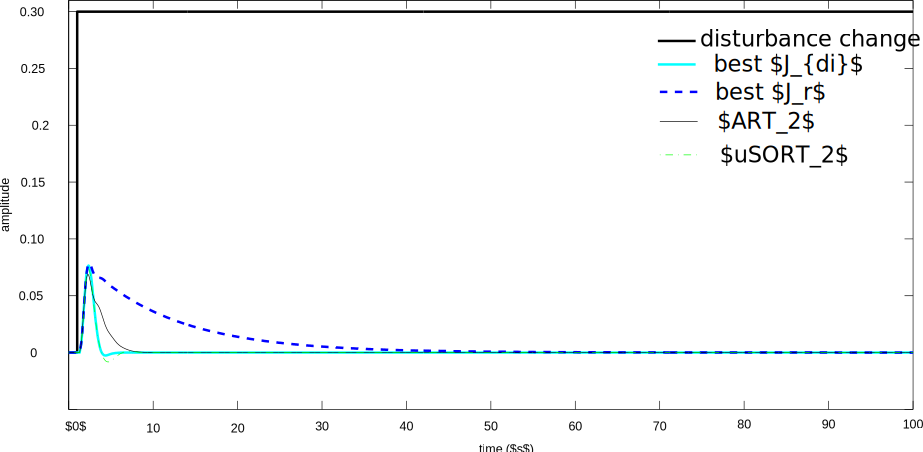
\includegraphics[width=\columnwidth]{cambiodi}%
	\caption{Optimal response of the control system $J_{di}$}%
	\label{fig:cambiodi}%
\end{figure}
%
%IAE ante cambio en valor de referencia
\begin{table}[tb]
	\caption{Servo response for the benchmark system.}
	\centering
	\begin{tabular}{@{}*{3}{c}@{}}
		\toprule
		Tuning             &IAE        &$M_s$   \\
		\midrule              
		optimum $J_{r}$     &$1.004$   & $2$    \\
		optimum $J_{di}$    &$1.297$   & $2$    \\
		$uSORT_2$          &$1.522$   & $2$    \\
		$ART_2$          &$2.121$   & $2$    \\	
		\bottomrule				
	\end{tabular}
	\label{tab:IAEref}
\end{table}
%
%IAE ante cambio en perturbación
\begin{table}[tb]
	\caption{Regulator response for the benchmark system.}
	\centering
	\begin{tabular}{@{}*{3}{c}@{}}
		\toprule
		Tuning            &IAE        &$M_s$   \\
		\midrule              
		optimum $J_{di}$   &$0.1017$   & $2$    \\
		$uSORT_2$          &$0.1095$   & $2$    \\
		$ART_2$            &$0.1574$    & $2$    \\	
		optimum $J_{r}$    &$0.8283$   & $2$    \\
		\bottomrule				
	\end{tabular}
	\label{tab:IAEdi}
\end{table}

It is important to note that in these figures, only two possible points (in fact, the two extreme cases) were considered, but in reality, there are much more options to select for intermediate values of the parameters between these two cases. It has to be noticed that the second order overdamped model is well suited to approximate high order models. Therefore, having done the computation for this particular model as presented in Section~\ref{sec:SolMOOP} allows to tackle almost any real-case of overdamped plants that can be found in the industry. The tool that was presented in Section~\ref{sec:DatabaseMOOP} is used in Section~\ref{sec:Description} with a more realistic industrial case.
%-----------------------------------------------------------------------------------------------------------------------------------
\section{LiTaO$_3$ Thin Film Deposition Process}
\label{sec:LiTAO3}
Temperature control is a very important factor in the deposition process of lithium tantalate (LiTaO$_3$) by means of metal organic chemical vapor deposition (MOCVD) \citep{Zhang2004}.

The dynamics of the reactor chamber are characterized by a large lag and time-delay. It is important for the quality of the final product, that the controller follow a predefined temperature profile accurately (servo control) while been able to reject other disturbances (regulatory control).

The model of the MOCVD chamber can be given by:
\begin{equation}
G(s) = \frac{K e^{-L s}}{T s+1},
\label{eq:GsLita}
\end{equation}
%
where the gain $K = 3.2$, the time constant $T = 200$~s and the time-delay $L = 150$~s.

For this case, a two function MOOP is considered with $J_{di}$ and $J_{r}$ as cost functions and a robustness restriction of $M_S = 2.0$. When solving the optimization using the ENNC method, the obtained Pareto front is as given in %
\begin{figure}[tb]
	\centering
	\begin{tikzpicture}
	\begin{axis}[
	xlabel = $J_{di}$,
	ylabel = $J_{r}$,
	grid = major,
	width=0.7\columnwidth,
	xtick={0.7,0.75,...,1.2},
	ytick={1.2,1.22,...,1.5},
	]
	\addplot[mark=none, line width=2pt,] table[x=Jdi, y=Jr]{./tablas/Pareto_LiTa_ms2.dat};
	\end{axis}
	\end{tikzpicture}
	\caption{Pareto front for the LiTaO$_3$ thin film deposition process.}
	\label{fig:LitaPareto}
\end{figure}
%
figure~\ref{fig:LitaPareto}.

Again, the Pareto front let the decision maker to choose between multiple possible solutions. In this particular case, taking the anchor point for minimum value of $J_{di}$ from Figure~\ref{fig:LitaPareto}, it can be seen that, from this point, if $J_{di}$ is degraded by $1.8\%$, it means an improvement of $4.37\%$ for $J_{r}$. This information could only be possible if the Pareto is available is some way, either as a graph or as a set of raw data.

In order to help the control engineer to understand the tuning of the controller, it could be useful to plot the variation of the controller parameters as a function of the degradation of one of the cost functions. Given that the LiTaO$_3$ Thin Film Deposition Process requires to follow a given temperature profile, the control engineer may surely consider $J_r$ as the main function.
%
\begin{figure}[tb]
	\centering
	\subfloat[$K_p$ variation for the LiTaO$_3$ thin film deposition process as a function of $J_r$ degradation.]{
	\begin{tikzpicture}
	\begin{axis}[
	label style={font=\scriptsize},
	tick label style={font=\scriptsize},
	xlabel = $m$ (\%),
	ylabel = $K_p$,
	grid = major,
	width=0.45\columnwidth,
	%scaled x ticks={real:0.01},
	%xtick scale label code/.code={},
	xtick={0,0.2,...,1.2},
	scaled x ticks={real:0.01},
	xtick scale label code/.code={},
	ytick={0.41,0.412,...,0.44},
	y tick label style={
		/pgf/number format/.cd,
		fixed,
		fixed zerofill,
		precision=3,
		/tikz/.cd
	}
	]
	\addplot[mark=none, line width=1pt,color=brown] table[x=Jrn, y=Kp]{./tablas/Pareto_LiTa_ms2.dat};
	\end{axis}
	\end{tikzpicture}
	\label{fig:LitaParetoKp}}\qquad
	%
	\subfloat[$T_i$ variation for the LiTaO$_3$ thin film deposition process as a function of $J_r$ degradation.]{
		\begin{tikzpicture}
		\begin{axis}[
		label style={font=\scriptsize},
		tick label style={font=\scriptsize},
		xlabel = $m$ (\%),
		ylabel = $T_i$,
		grid = major,
		width=0.45\columnwidth,
		xtick={0,0.2,...,1.2},
		scaled x ticks={real:0.01},
		xtick scale label code/.code={},
		%xtick={0,0.1,...,1},
		ytick={200,220,...,320},
		]
		\addplot[mark=none, line width=1pt,color = blue] table[x=Jrn, y=Ti]{./tablas/Pareto_LiTa_ms2.dat};
		\end{axis}
		\end{tikzpicture}
		\label{fig:LitaParetoTi}
		}\\
	%
	\subfloat[$T_d$ variation for the LiTaO$_3$ thin film deposition process as a function of $J_r$ degradation.]{
		\begin{tikzpicture}
		\begin{axis}[
		label style={font=\scriptsize},
		tick label style={font=\scriptsize},
		xlabel = $m$ (\%),
		ylabel = $T_d$,
		grid = major,
		width=0.45\columnwidth,
		xtick={0,0.2,...,1.2},
		scaled x ticks={real:0.01},
		xtick scale label code/.code={},
		%xtick={0,0.1,...,1},
		ytick={40,41,...,55},
		]
		\addplot[mark=none, line width=1pt,color = red] table[x=Jrn, y=Td]{./tablas/Pareto_LiTa_ms2.dat};
		\end{axis}
		\end{tikzpicture}
		\label{fig:LitaParetoTd}
		}\qquad
	%
	\subfloat[$\beta$ variation for the LiTaO$_3$ thin film deposition process as a function of $J_r$ degradation.]{
		\begin{tikzpicture}
		\begin{axis}[
		label style={font=\scriptsize},
		tick label style={font=\scriptsize},
		xlabel = $m$ (\%),
		ylabel = $\beta$,
		grid = major,
		width=0.45\columnwidth,
		xtick={0,0.2,...,1.2},
		scaled x ticks={real:0.01},
		xtick scale label code/.code={},
		%xtick={0,0.1,...,1},
		ytick={0.65,0.7,...,1.05},
		]
		\addplot[mark=none, line width=1pt,color = olive] table[x=Jrn, y=beta]{./tablas/Pareto_LiTa_ms2.dat};
		\end{axis}
		\end{tikzpicture}
		\label{fig:LitaParetoBeta}	
	}
	%
	\caption{Variation of the parameters vs $J_r$ for the  LiTaO$_3$ thin film deposition process.}
	\label{fig:LitaParetoParam}
\end{figure}
%

In Figure~\ref{fig:LitaParetoParam} the values of all the controller parameters are plotted against $m$, where $m$ is defined as the normalized degradation of $J_{r}$ ($m=0$ represents the anchor point where $J_r$ has its lowest value). Looking the behaviour of $K_p$ in Figure~\ref{fig:LitaParetoKp}, it is clear that the value of $K_p$ is kept fairly constant for all values of $m$. This almost negligible variation may be associated to the fact that, for all controller tunings, the maximum sensitivity is set at $M_S = 2$. When this constraint is not taken into account, the value of $K_p$ may have large variations as in the example in Section~\ref{sec:CSTH}.

For the case of the integral time $T_i$, the behavior of this parameter is plotted in Figure~\ref{fig:LitaParetoTi}. Note that, contrary to the case of $K_p$, the variation is highly dependent of $J_r$ and fairly smooth, which is desirable if the interest is to find a tuning rule. However, for the derivative time $T_d$ in Figure~\ref{fig:LitaParetoTd}, it can be seen that the variation is important but the behavior is not as near as smooth as in the case of $T_i$. Finally and the setpoint weight factor $\beta$, also has a piece-wise behavior with respect to $J_r$ and also the variation of its value is important. Nevertheless, once computed the corresponding tunings of all the controllers of the Pareto, is just to pick and decide which one is more appropriate for the task.

The response of the controlled system to a setpoint step change is presented in %
%
\begin{figure}[tb]
	\centering
	\begin{tikzpicture}
	\begin{axis}[
	label style={font=\scriptsize},
	tick label style={font=\scriptsize},
	xlabel = time~(s),
	ylabel = output,
	legend cell align=left,
	legend style = {legend pos = south east, font=\scriptsize},%{at={(1,0.05)}, anchor=south east},%
	grid = major,
	width=\columnwidth,
	%scaled x ticks={real:0.01},
	%xtick scale label code/.code={},
	xtick={0,200,...,1600},
	%ytick={41,42,...,52},
	]
	\addplot[mark=none, color=red] table[x=time, y=r]{./tablas/TestServo.dat};
	\addplot[mark=none,dashed, color=blue] table[x=time, y=yservo]{./tablas/TestServo.dat};
	\addplot[mark=none,densely dashdotdotted, color=olive] table[x=time, y=yreg]{./tablas/TestServo.dat};
	\addplot[mark=none,dashdotted, color=magenta] table[x=time, y=yusort]{./tablas/TestServo.dat};
	\legend{Reference,$m=0\%$ (IAE=$244.66$), $m=100\%$ (IAE=$285.64$),uSORT$_2$ (IAE=$304.39$)}
	\end{axis}
	\end{tikzpicture}
	\caption{Servo response of the LiTaO$_3$ thin film deposition process with tree different tuning.}
	\label{fig:LitaServo}
\end{figure}
%
figure~\ref{fig:LitaServo} and for a step signal in the input disturbance in %
%
\begin{figure}[tb]
	\centering
	\begin{tikzpicture}
	\begin{axis}[
	label style={font=\scriptsize},
	tick label style={font=\scriptsize},
	xlabel = time~(s),
	ylabel = output,
	legend cell align=left,
	legend style = {at={(1.05,1)}, anchor=north east, font=\scriptsize},%{legend pos = north east},%
	grid = major,
	width=\columnwidth,
	%scaled x ticks={real:0.01},
	%xtick scale label code/.code={},
	xtick={0,200,...,1600},
	%ytick={41,42,...,52},
	]
	\addplot[mark=none, color=red] table[x=time, y=di]{./tablas/TestReg.dat};
	\addplot[mark=none,dashed, color=blue] table[x=time, y=yservo]{./tablas/TestReg.dat};
	\addplot[mark=none,densely dashdotdotted, color=olive] table[x=time, y=yreg]{./tablas/TestReg.dat};
	\addplot[mark=none,dashdotted, color=magenta] table[x=time, y=yusort]{./tablas/TestReg.dat};
	\legend{Disturbance, $m=0\%$ (IAE=$724.24$), $m=100\%$ (IAE=$502.65$),uSORT$_2$ (IAE=$522.00$)}
	\end{axis}
	\end{tikzpicture}
	\caption{Regulation response of the LiTaO$_3$ thin film deposition process with tree different tuning.}
	\label{fig:LitaReg}
\end{figure}
%
figure~\ref{fig:LitaReg}. For both cases, the anchor points controllers where compared against the uSORT$_2$ tuning rule \citep{Alfaro2012}, since both uses a \gls{2dof} \gls{pid} controller structure and both attempt to minimize an \gls{iae} cost function.

Take into account the response presented in Figure~\ref{fig:LitaServo}. The response of the controlled system is compared against the uSORT$_2$ method as in Section~\ref{sec:Bechmark} given that in this particular example the value of \gls{ms} is also considered. Given that the responses taken from the Pareto are the extreme cases, it is to be expected that all other responses in the Pareto are going to be between these two. Therefore, all the controllers in the Pareto surpass the servo response of the uSORT$_2$, which is not a surprising result given that the uSORT$_2$ method is said to be suboptimal with respect to the servo response, as it is primarily optimized for regulation.

For this same reason, when examining the responses in Figure~\ref{fig:LitaReg} for the disturbance rejection case, it can be seen that the uSORT$_2$ response is close to the case of $m = 100\%$ and this is exactly what it was expected since the uSORT$_2$ method was intended for regulation. Of course, the tuning of the other anchor point has a much worse response, and therefore, the uSORT$_2$ response lies between these two extremes. However, this fact does not mean that the uSORT$_2$ method is optimal in the Pareto sense, because, it may  be possible to find a better servo response with a similar regulation \gls{iae}.

Finally to consciously be aware of the advantage of computing the Pareto front, in %
%
\begin{figure}[tb]
	\centering
	\begin{tikzpicture}
	\begin{axis}[
	label style={font=\scriptsize},
	tick label style={font=\scriptsize},
	xlabel = time~(s),
	ylabel = output,
	legend cell align=left,
	legend style = {legend pos = south east, font=\scriptsize},%{at={(1,0.05)}, anchor=south east},
	grid = major,
	width=\columnwidth,
	%scaled x ticks={real:0.01},
	%xtick scale label code/.code={},
	xtick={0,200,...,1600},
	%ytick={41,42,...,52},
	]
	\addplot[mark=none, color=red] table[x=time, y=y1.00]{./tablas/TestParetoServo.dat};
	\addplot[mark=none,dashed, color=blue] table[x=time, y=y0.61]{./tablas/TestParetoServo.dat};
	\addplot[mark=none,densely dashdotdotted, color=olive] table[x=time, y=y0.31]{./tablas/TestParetoServo.dat};
	\addplot[mark=none,dotted, color=magenta] table[x=time, y=y0.12]{./tablas/TestParetoServo.dat};
	\addplot[mark=none,dashdotted, color=cyan] table[x=time, y=y0.00]{./tablas/TestParetoServo.dat};
	\legend{$m=100\%$, $m=61\%$,$m=31\%$,$m=12\%$,$m=0\%$}
	\end{axis}
	\end{tikzpicture}
	\caption{Servo response of the LiTaO$_3$ thin film deposition process varying the tuning across the Pareto front with different degradations.}
	\label{fig:LitaServoParetoResp}
\end{figure}
%
figure~\ref{fig:LitaServoParetoResp}, five points of the Pareto front where selected ranging from $m=100\%$ to $m=0\%$ and the reference tracking response was plot in the same axis. As before, the front was found with the constraint $M_{S,max}\leq 2.0$. The fact that, among all possible controllers computed, at the end only one of them is going to be selected, may  be seen as a ``waste'' of resources. And this surely may be true if the Pareto is computed for every single case. However, if a general case is computed beforehand and a tool is used to select one of the many controllers, the Pareto front then can be seen more advantageous and certainly more useful for the decision maker. An example of such case is presented in Section~\ref{sec:PIDCSTH}. 
%-----------------------------------------------------------------------------------------------------------------------------------
%
\section{Continuous stirred tank heater}
\label{sec:CSTH}
%
\subsection{Description of the process}
\label{sec:Description}
%
The control of a \gls{csth} is a common task in industrial processes. In this section, the control of the temperature of the \gls{csth} will be solved as a \gls{moop} using a \gls{2dof} \gls{pid} controller. The diagram of the process is presented in %
\begin{figure}[b]
	\centering
	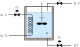
\includegraphics{Ch7CSTR}
	\caption{Simplified diagram of a continuous stirred-tank heater to be controlled.}
	\label{fig:Ch7CSTR}
\end{figure}
Figure~\ref{fig:Ch7CSTR}. A heat exchanger is installed inside the tank to heat the fluid. The flow rate inside the heat exchanger is controlled with a valve with input variable $U_T$ and the liquid inside the heat exchanger enters with temperature $T_{ci}$ and leaves with temperature $T_{co}$, the average temperature inide the heat exchanger is $T_{ca}$. The volume inside the tank is variable, the input flow rate is $Q_i$ with temperature $T_i$. The output flow rate is $Q$ with temperature $T$. The output flow rate is controlled with a valve with input variable $U_L$. The tank is covered with a jacket that prevents any heat loss to the atmosphere.

According to \citet{Alfaro2016}, a possible model for this process is given by the following set of algebraic-differential equations:
\begin{itemize}
	\item Tank mass balance:
			\begin{equation*}
				A \frac{d H(t)}{dt} = Q_i(t) - Q(t),
			\end{equation*}
			where $A$ is the transversal area of the tank and $H(t)$ is the liquid level.
	\item Tank energy balance:
			\begin{equation*}
				\rho C_p A H(t) \frac{T(t)}{dt} = \rho C_p Q_i(t)\left( T_i(t) - T(t)\right) + W(t),
			\end{equation*}
			where $C_p$ is the heat capacity of the fluid and $W(t)$ is the rate of heat transfer from the heat exchanger to the tank. $W(t)$ can be modeled as:
	\item Heat exchanger energy balance:
			\begin{equation*}
				\rho_c C_{pc} V_c \frac{T_{ca}(t)}{dt} = \rho_c C_{pc} Q_c(t)\left( T_{ci}(t)-T_{co}(t)\right) - W(t),
			\end{equation*}
			where $\rho_c$ is the density of the fluid inside the heat exchanger, $C_{pc}$ is the heat capacity of the fluid inside the heat exchanger and $V_c$ is the volume of the heat exchanger.
	\item Heat transfer between the heat exchanger and the fluid in the tank:
			\begin{equation*}
				W(t) = U A_c \left( T_{ca}(t) - T(t)\right), 
			\end{equation*}
			where $U$ is overall heat-transfer coefficient, $A_c$ is the area of the heat exchanger, $T_{ca}(t)$ is the average temperature inside the heat exchanger which is related to $T_{co}(t)$ and $T_{ci}(t)$ as:
			\begin{equation*}
				T_{ca}(t) = \frac{T_{ci}(t) + T_{co}(t)}{2}
			\end{equation*}
\end{itemize}

Also, in \citet{Alfaro2016}, the transmitters and the valves are modeled as:
\begin{itemize}
	\item Level transmitter: it is supposed that the level transmitter is a capacitive type electronic transmitter that has a first order dynamics:
		\begin{equation*}
			T_L \frac{d Y_L(t)}{dt} + Y_L(t) = K_L H(t),
		\end{equation*}
		%
		where $T_L$ is its time constant, $Y_L$ is the level signal and $K_L$ is the transmitter gain.
	%
	\item Temperature transmitter: It is supposed that a Pt$_{100}$ RTD electronic sensor is installed in a thermowell at the tank outlet pipe. It is supposed that it has a second order dynamic:
	%
		\begin{equation*}
			T_{T}^2 \frac{d^2 Y_T(t)}{dt^2} + 2T_T \frac{d Y_T(t)}{dt} + Y_T(t) = K_T T(t),
		\end{equation*}
		%
		where $T_T$ is its time constant and $K_T$ is its gain.
	%
	\item Level control valve: it is supposed that a ball valve with an electroneumatic actuator is used. The valve	inherent flow characteristics is nearly quadratic and the relationship between the flow $Q(t)$ and the input variable $U_L$ is given by:
		\begin{align*}
			T_{vL} \frac{d X_L(t)}{dt} + X_L(t) = K_{xL} U_L(t),\\
			Q(t) = K_{vL} X_L^2(t)\sqrt{\rho g H(t)},
		\end{align*}
		where $T_{vL}$ is the level control valve time constant, $K_{xL}$ level control valve stem constant $K_{vL}$ level control valve constant and $X_L(t)$ is the level control valve stem normalized travel.
	%
	\item Temperature control valve it is also supposed to be a ball valve with an electroneumatic actuator, however, it is supposed that the valve has an equal-percentage inherent flow characteristics given by:
		\begin{align*}
			T_{vT} \frac{d X_T(t)}{dt} + X_T(t) = K_{xT} U_T(t),\\
			Q_c(t) = K_{vT}R_{vT}^{\left( X_T(t) -1 \right) } \sqrt{P_{cp} - \left(R_c Q^2_c(t)+P_{cr} \right) },
		\end{align*}
		where $T_{vT}$ is the temperature control valve time constant, $K_{xT}$ the temperature control valve stem constant, $K_{vT}$ is the temperature control valve constant $P_{cp}$ is the heating fluid pump discharge pressure, $P_{cr}$ is heating fluid system return pressure and $X_T(t)$ is the temperature control valve stem normalized travel.
\end{itemize}

Taking this model in consideration, it can be said that, from the point of view of the controller, the controlled variables are give by the signals $Y_L(t)$ (which represents the level) and $Y_T(t)$ (which represents the temperature of the fluid of the tank). The manipulated variables are given by $U_L(t)$ (which directly affects $Q$) and $U_T(t)$ (that directly affects $Q_{c}$). $Q_i(t)$, $T_i$ and $T_{ci}$ are considered as disturbances. The state variables of the system are given by $H(t)$, $T_T(t)$, $T_{co}$, $Y_L(t)$, $Y_T$, $X_L(t)$ and $X_T(t)$, therefore, this model comprises a seventh order non-linear system for a two-input two-output industrial process. The parameters of the model can be found in 
\begin{table}
	\centering
	\caption{Parameters for the CSTH process}
	\label{tab:ParametersCSTH}
	\begin{tabular}{ccc}
		\toprule
		\textbf{Symbol} & \textbf{Value} & \textbf{Description}\\
		\midrule
		\multicolumn{3}{c}{\textbf{\textit{Tank parameters}}}\\
		\midrule
		$\rho$ 		& \SI{1200}{\kilogram\per\meter\cubed} 			& tank fluid density\\
		$A$			& \SI{0.0707}{\square\meter}					& tank inside section area\\
		$C_p$		& \SI{4190}{\joule\per\kilogram\per\celsius}	& tank fluid heat capacity\\
		$g$			& \SI{9.8}{\meter\per\square\second}			& gravity acceleration\\
		$K_T$		& \SI{2}{\%\per\celsius}						& temperature transmitter gain\\
		$K_{vL}$	& \num{1.25e-5}									& level control valve constant\\
		$K_{vT}$	& \num{3e-6}									& temperature control valve constant\\
		$K_{xL}$	& \SI{0.01}{\per\%}								& level control valve stem constant\\
		$Q_i$		& \SI{7e-4}{\cubic\meter\per\second}			& normal tank inlet fluid flow rate\\
		$T_i$		& \SI{24}{\celsius}								& fluid inlet temperature\\
		$T_L$		& \SI{2}{\second}								& level transmitter time constant\\
		$T_T$		& \SI{15}{\second}								& temperature transmitter time constant\\
		$T_{vL}$	& \SI{3}{\second}								& level control valve time constant\\
		$T_{vT}$	& \SI{5}{\second}								& temperature control valve time constant\\
		\midrule
		\multicolumn{3}{c}{\textbf{\textit{Heat exchanger parameters}}}\\
		\midrule
		$\rho_c$ 	& \SI{800}{\kilogram\per\meter\cubed} 			& heating fluid density\\
		$A_c$		& \SI{0.6362}{\square\meter}					& heat exchanger transfer area\\
		$C_{pc}$	& \SI{2400}{\joule\per\kilogram\per\celsius}	& heating fluid heat capacity\\
		$K_L$		& \SI{125}{\%\per\meter}						& level transmitter gain\\
		$K_{xT}$	& \SI{0.01}{\per\%}								& temperature control valve stem constant\\
		$P_{cp}$	& \SI{4.14e5}{\pascal}							& heating fluid pump discharge pressure\\
		$P_{cr}$	& \SI{1.38e5}{\pascal}							& heating fluid system return pressure\\
		$R_c$		& \SI{5.5e10}{\pascal\per(\cubic\meter\per\second)^2}	& heating system pipe nominal flow resistance\\
		$R_{vT}$	& \num{50}										& temperature control valve rangeability\\
		$T_{ci}$	& \SI{320}{\celsius}							& heating fluid inlet temperature\\
		$U$			& \SI{440}{\joule\per\second\per\square\meter\per\celsius}	& overall heat-transfer coefficient\\
		$V_c$		& \SI{0.0139}{\cubic\meter}						& heat exchanger volume\\
		\bottomrule
	\end{tabular}
\end{table}
%
Table~\ref{tab:ParametersCSTH}. This model was implemented in Simulink and can be found with the companion software. In %
%
\begin{figure}[tb]
	\centering
	\includegraphics[width=\columnwidth]{Ch7Implementation}
	\caption{Simulink implementation of the model of the heater.}
	\label{fig:Ch7Implementation}
\end{figure}
%
Figure~\ref{fig:Ch7Implementation}. Each equation of the model was implemented in a subsystem for clarity. For example in %
\begin{figure}
	\centering
	\includegraphics[width=\columnwidth]{Ch7HeatExhangerEq}
	\caption{Example of the implementation of the heat exchanger energy balance.}
	\label{fig:Ch7HeatExhangerEq}
\end{figure}
%
Figure~\ref{fig:Ch7HeatExhangerEq} the Simulink implementation of the heat exchanger energy balance is presented. The result of this submodel is the computation of the state variable $T_{ca}$, which represents the average temperature of the heating fluid. As it can be seen, the parameters of the model are not hard-coded in the Simulink blocks, instead a parameter initialization script is call before the simulation starts. If the user desires to change any value of the parameters, it can be done globally in the script and then automatically called during the simulation.

\subsection{Simplified linear model}
\label{sec:SimpLinMod}
In order to find a PID controller using the MOOTuning app, it is necessary to find a linear model of the plant in the operation point. An identification procedure was performed with a change of 10\% in the value of $U_T$ to find the transfer function between $Y_T$ and $U_T$. The response to this change is depicted in %
\begin{figure}[tb]
	\centering
	\includegraphics[width=\columnwidth]{Ch7CSTHResp}
	\caption{Response of the process to a change of 10\% in the $U_T(t)$ input.}
	\label{fig:Ch7CSTHResp}
\end{figure}
%
Figure~\ref{fig:Ch7CSTHResp}. As it can be seen, the response is overdamped and takes approximately \SI{500}{\second} to reach a new steady state. A change in 10\% on the input signal produces a variation of approximately $3.5\%$ in the output signal. It has to be noticed that the presented signals are normalized between 0 and 100\% representing the full spam of the transmitter and actuators.

In order to find the model, the process was supposed to have two poles, no zeros and a pure time-delay (also known as dead-time). Of course, if a linearization procedure were performed using the nonlinear model, a seventh order model would be obtained. However, for PID tuning, a first or second order model is usually expected to tune the controller.

Considering the experiment performed with the data as depicted in Figure~\ref{fig:Ch7CSTHResp}, the resulting simplified model is given by:
%
\begin{equation}
\frac{Y_T(s)}{U_T(s)} = \frac{0.3658 e^{-24.736 s}}{(52.861 s+1)(52.805 s +1)}.
\label{eq:TFCSTH}
\end{equation}

From this transfer function, it can be deduced that the gain is equal to $K = 0.3658$, the main time constant is given by $T = 52.861$, the ratio between the two time constant is given by $a = 0.9989$ and the dead-time is given by $L = 24.736$, therefore the normalized dead-time is given by $\tau = 0.4679$.

To test the validity of this simplified model, the response of the transfer function is compared against the response of the non-linear model. It was found that the transfer function response is very similar to the response of the non-linear model, as can be seen in %
%
\begin{figure}[tb]
	\centering
	\includegraphics[width=\columnwidth]{Ch7CSTHComp}
	\caption{Comparison between the linear and no linear models for the CSTH.}
	\label{fig:Ch7CSTHComp}
\end{figure}
%
Figure~\ref{fig:Ch7CSTHComp}. It is clear that the non-linear model is a good representation of the dynamical response of the process. This is the first step in order to find a suitable PID controller to control the plant. In \citet{Alfaro2016} the level of the tank is also controlled, however the dynamic of the level is simpler (its model can be approximated with a first order model without delay) and in this particular example, only the temperature is going to be controlled, while the level is considered to be constant.
%
\subsection{PID control of the CSTH considering two integral cost functions}
\label{sec:PIDCSTH}
In this section, the process will be controlled using a \gls{pid} controller with different tuning methods and compared with the \gls{moo} framework used in the book.

Two different tuning rules were considered: the method by \citet{Rovira1969a} and the method by \citet{Murril1967}. For the case of the Rovira and Murril method, the model in \eqref{eq:TFCSTH} was reduced to a first order model using the Half-Rule in \citet{Skogestad2003}:
\begin{equation}
\frac{Y_T(s)}{U_T(s)} = \frac{0.3658 e^{-24.7360 s}}{79.2635 s +1}.
\label{eq:TFCSTHFirstOrder}
\end{equation}

The equations were implemented as presented in \citet{odwyer2006}:
\begin{itemize}
%	\item SIMC method: Supposing a \gls{soptd} model:
%			\begin{equation*}
%				P(s) = \frac{K e^{-Ls}}{(Ts+1)(aTs+1)}
%			\end{equation*}
%			The corresponding PID tuning for a closed-loop lag time of $T_c = L$ and the case where $T \leq 8 L$, the PID tuning is given by:
%			\begin{align*}
%				K_p &= \frac{0.5}{K}\frac{(1+a)T}{L}\\
%				T_i &= (1 + a) T\\
%				T_d	&= \frac{a}{1+a}T
%			\end{align*}
%	%
	\item Supposing a \gls{foptd} model given by:
			\begin{equation*}
				P(s) = \frac{K e^{-L s}}{Ts+1}
			\end{equation*}
			The Murrill tuning is given by:
				\begin{align*}
					K_p &= \frac{1.435}{K}\left( \frac{T}{L} \right)^{0.921}\\
					T_i &= \frac{T}{0.878}\left( \frac{L}{T}\right)^{0.749}\\\\
					T_d &= 0.482 T \left( \frac{L}{T} \right)^{1.137}
				\end{align*}
	\item Again, supposing a \gls{foptd} as above, the Rovira tuning is given by:
			\begin{align*}
				K_p &= \frac{1.086}{K} \left( \frac{T}{L}\right) ^{0.869} \\
				T_i &= \frac{T}{0.740 - 0.13\frac{L}{T}} \\
				T_d &= 0.384 T \left( \frac{L}{T}\right)^{0.914} 
			\end{align*}
\end{itemize}

The values of the computed values can be found on %
\begin{table}[tb]
	\centering
	\caption{Comparison of different PID tunings for the CSTH process.}
	\setlength{\tabcolsep}{8pt}
	\begin{tabular}{ccccccc}
		\toprule
		Tuning 	& $K_p$ 	& $T_i$		& $T_d$		& $\beta$	& $J_{r}$	& $J_{di}$\\
		\midrule
		%
		%SIMC	& $5.84$	& $105.67$	& $26.42$	& $1$			& $55.14$	& $18.10$\\
		Murril	& $5.87$	& $65.02$	& $23.21$	& $1$			& $82.51$	& $15.34$\\
		Rovira	& $4.34$	& $120.81$	& $18.48$	& $1$			& $76.00$	& $27.79$\\
		MOO01	& $11.3$	& $58.82$	& $29.48$	& $0.43$		& $85.65$	& $7.06$\\
		MOO02	& $9.26$	& $123.85$	& $26.68$	& $0.80$		& $69.96$	& $13.38$\\
		MOO03	& $8.20$	& $185.21$	& $28.14$	& $0.99$		& $67.93$	& $22.54$\\
		\bottomrule
	\end{tabular}
	\label{tab:CompPIDCSTH}
\end{table}
%
Table~\ref{tab:CompPIDCSTH}, along with its associated values of $J_{di}$ and $J_r$. The Murril and Rovira methods presented in the table were selected because they are intended to minimize the \gls{iae}. In all cases, the PID tuning is for a one degree of freedom controller (that is  the reason why $\beta$ is equal to one).

The PID that can be found using the data and the framework presented in Chapter~\ref{chap:PIDMOOP} is a \gls{soptd}, which may do the comparison somehow unfair. However, the idea now is to compare methods that tries to minimize the \gls{iae}. Using the MOOTuning Tool that accompanies this book, the Pareto front that was found is given as in %
%
\begin{figure}[tb]
	\centering
	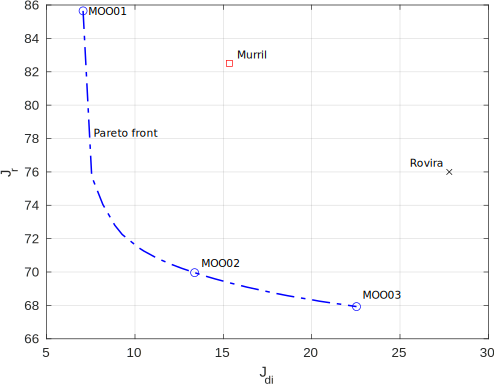
\includegraphics[width=\columnwidth]{Ch7CompPareto}
	\caption{MOOTuning compared to the Murril and Rovira methods that also minimizes \gls{iae}.}
	\label{fig:Ch7CompPareto}
\end{figure}
%
Figure~\ref{fig:Ch7CompPareto}. As it was expected, all the controllers found using the \gls{moo} tool present lower values for $J_{di}$ and $J_r$. If all controllers had the same topology, most certainly both controller would be close to the anchor points. However, what it is important here is the fact that, using the tool, the user has the ability to chose between practically an infinity of possible controllers. From the Pareto front, three different tuning were selected in order to compare the responses using the non-linear plant. The values of the parameters are presented also in Table~\ref{tab:CompPIDCSTH} and depicted as circles in the Pareto front in Figure~\ref{fig:Ch7CompPareto}.
%
\begin{figure}[tb]
	\centering
	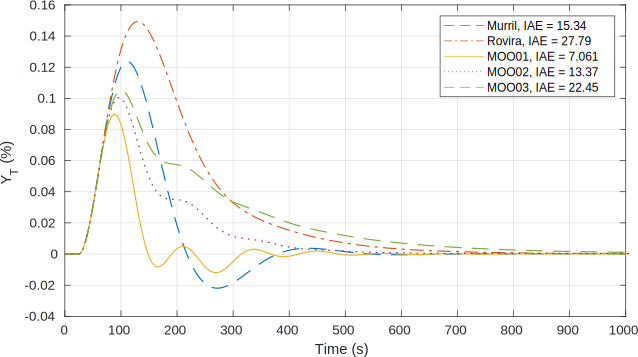
\includegraphics[width=\columnwidth]{Ch7CompParetoReg}
	\caption{Regulator response comparison for minimum IAE.}
	\label{fig:Ch7CompParetoReg}
\end{figure}
%
\begin{figure}[tb]
	\centering
	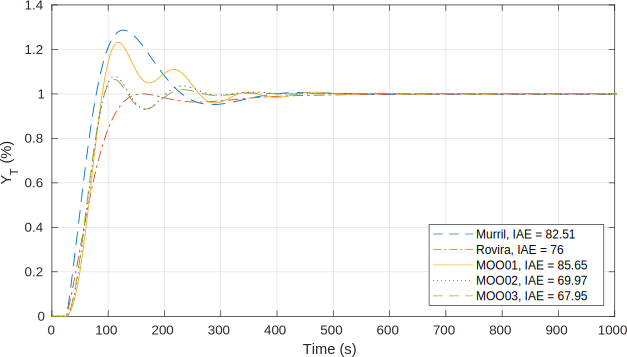
\includegraphics[width=\columnwidth]{Ch7CompParetoServo}
	\caption{Servo response comparison for minimum IAE.}
	\label{fig:Ch7CompParetoServo}
\end{figure}

In Figures~\ref{fig:Ch7CompParetoReg} and \ref{fig:Ch7CompParetoServo} the responses to a step change in the setpoint and in the disturbance are presented. The corresponding values of \gls{iae} are also presented in the graph. In all cases, the robustness was not considered as a constraint. but it is possible to include it within the MOOTuning software. From Figure~\ref{fig:Ch7CompPareto} given the steep slope of the curve for lower values of $J_{di}$ that a small change in $J_{di}$ may improve substantially the performance for $J_r$. Therefore, one may be more prone to select a controller that may have a little degradation in $J_{di}$ and for this reason, controller MOO01 may not be a good selection as a final solution unless having the minimum value possible of $J_{di}$ is the final goal.

The controller MOO02 may be seen as an intermediate solution between MOO1 and MOO03 in case both $J_{di}$ and $J_r$ are equally important for the decision maker. The power of the multiobjective framework is evident, and giving that the computational power is done offline, it becomes a good tool for the tuning of PIDs in an industrial setting.

To check how the tuning performs with the nonlinear model, a simulation was performed using the tuning of the controller $MOO02$. The setpoint was increased by $5\%$ at $t=\SI{100}{\second}$ and the temperature of the steam was increased by $\SI{10}{\celsius}$ at $t=\SI{700}{\second}$. The response is presented in %
\begin{figure}[tb]
	\centering
	\includegraphics[width=\columnwidth]{Ch7CSTRControlled}
	\caption{Response of the controlled system using the nonlinear model for the CSTH.}
	\label{fig:Ch7CSTRControlled}
\end{figure}
%
Figure~\ref{fig:Ch7CSTRControlled}. As it can be seen, the servo response is very close to the one presented in Figure~\ref{fig:Ch7CompParetoServo}, which is a clear indicator that the linear model was a good approximation of the plant at the given operation point. The response to the change in the stem temperature cannot be compared with the regulation presented in Figure~\ref{fig:Ch7CompParetoReg}, because the disturbance was not applied directly in the input of the plant. However, it is interesting to note that the controller was able to respond with a good dynamic even though it was not optimize for this case.

The controlled variable is presented in %
\begin{figure}[tb]
	\centering
	\includegraphics[width=\columnwidth]{Ch7CSTRControlledCV}
	\caption{Response of the controlled system using the nonlinear model for the CSTH.}
	\label{fig:Ch7CSTRControlledCV}
\end{figure}
%
Figure~\ref{fig:Ch7CSTRControlledCV}. When the setpoint change, the response of the controller is abrupt (more than double its original value), but then the value rapidly reach the new setpoint. The change produced by the disturbance has a milder response, and in less than \SI{200}{\second} reach again a new steady state.

The case presented here tried to show the steps to use the Pareto front as the methodology to find the controller tuning more appropriate to the task. The example is a simple plant, but very representative of the dynamics that can be found in an industry environment. Many of the plants can be modeled as a second order overdamped process, and therefore, the tool and the data used in this book are readily applied in many cases.

\subsection{PID control of the CSTH considering three integral cost functions}
\label{sec:PIDCSTH3Fun}
The MOOTuning software also is able to find the optimal parameters of a PID controllers considering three cost functions as presented in Section~\ref{sec:Tuning3PID}. Of course, it is not necessary to use this software since the data base with all the values is also part of the companion software, but the \matlab{} app has the advantage to be a simple interface between the user and the data.

As an example, the tuning tool is used to find the parameters of the controller that has the lowest $J_{do}$ value. This case is interesting because the anchor point where $J_{do}$ has the lowest value, neither the value of $J_r$ nor $J_{di}$ have their maximum value. On the other hand, when $J_{r}$ is set to be the lowest possible value, $J_{do}$ becomes the function that has an intermediate value but $J_{di}$ has its maximum value from the Pareto. Only for the anchor point where $J_{di}$ is minimum, both $J_r$ and $J_{do}$ get their maximum value. The responses for the three anchor points are depicted %
\begin{figure}[tb]
	\centering
	\includegraphics[width=\columnwidth]{Ch7CSTHControlled3Fun}
	\caption{Response of the CSTH process in the three anchor points of the pareto front for $M_s \leq 2.0$.}
	\label{fig:Ch7CSTHControlled3Fun}
\end{figure}
%
in Figure~\ref{fig:Ch7CSTHControlled3Fun} for the case where $M_s \leq 2.0$. As it can be seen, the response is quite different among the three anchor points. First a change in the reference value is performed at $t=\SI{100}{\second}$, an input step disturbance is present at $t=\SI{1000}{\second}$ and an output step disturbance is introduced in the system at $t=\SI{2000}{\second}$. The values of the cost functions are presented in %
%
\begin{table}
	\centering
	\caption{Cost functions for the three cost functions case scenario.}
	\begin{tabular}{cccc}
		\toprule
		 				& $J_r$ anchor point 					& $J_{di}$ anchor point				&	$J_{do}$ anchor point	\\
		 \midrule
		 $J_r$			&		$67.95$	(minimal)				&		$85.63$	($+26.02\%$)		&	$82.46$($+21.35\%$) \\
		 $J_{di}$		&		$22.46$ ($+218.13\%$)			&		$7.06$	(minimal)			&	$17.63$ ($+149.72\%$)	\\
		 $J_{do}$		&		$74.25$ ($+38.01\%$)			&		$102.43$ ($+90.39\%$)		&	$53.80$	(minimal)				\\
		 Parameters		& \begin{tabular}{c} $K_p = 8.19$ \\ $T_i = 185.18$\\ $T_d = 28.14$\\ $\beta = 0.99$		 \end{tabular} &
		 \begin{tabular}{c} $K_p = 11.29$ \\ $T_i = 58.8306$\\ $T_d = 29.48$\\ $\beta = 0.43$ \end{tabular} &
		 \begin{tabular}{c} $K_p = 6.18$ \\ $T_i = 108.76$\\ $T_d = 29.93$\\ $\beta = 0.82$ \end{tabular}\\
		 \bottomrule
	\end{tabular}
	\label{tab:2FunCostFunctionCSTH}
\end{table}
%
Table~\ref{tab:2FunCostFunctionCSTH}. The percentage increment is reported for each cost function in each case.

Using Figure~\ref{fig:Ch7CSTHControlled3Fun} and Table~\ref{tab:2FunCostFunctionCSTH} , it can be confirmed that the tuning with the best parameters for $J_{di}$ produces the worst responses for the other two functions. With these results one may be prone to select the tuning for the lowest value of $J_{di}$ as the final because it does not have the worst values of the other cost functions and it has much better response for the output disturbance case. Observe for example the response for the $J_{di}$ anchor point where the response for the output disturbance is bad (it has a $J_{do}$ increment of $+90.39\%$ with respect to its lowest value). In some sense, it could be seen as the best compromise between the cost functions. Only if the control engineer is heavily invested in minimize the $J_{di}$ cost function, it may select the $J_{di}$ anchor point as the final response, however, using the multiobjective framework presented here, he or she has to be fully aware that is selecting the worst response for the other functions.

Another reason to select the $J_{do}$ anchor point is related to the control effort. When the Total Variation computed as:
\begin{equation*}
TV = \sum_{i=0}^{N-1}\left(  u(i+1)-u(i)\right),
\end{equation*}
is compared between the three responses, it is found that $TV_{J_r} = 223.82$, $TV_{J_{di}} = 352.94$ and $TV_{J_{do}} = 152.81$ using a step size of $\SI{0.01}{\second}$. It is clear that the response given by the $J_{do}$ anchor point is a very good choice among all the possible values. The control signal is plotted %
%
\begin{figure}[tb]
	\centering
	\subfloat[Reference and input disturbance step changes.]{\includegraphics[width=\columnwidth]{Ch7CSTHControlledCV3Fun01} \label{fig:Ch7CSTHControlledCV3Fun01}}\\
	\subfloat[Output disturbance step change.]{\includegraphics[width=\columnwidth]{Ch7CSTHControlledCV3Fun02} \label{fig:Ch7CSTHControlledCV3Fun02}}
	\caption{Control signal for the CSTH using three cost functions.}
	\label{fig:Ch7CSTHControlledCV3Fun}
\end{figure}
%
on Figure~\ref{fig:Ch7CSTHControlledCV3Fun}. Since the control signal has a larger magnitude for an output disturbance rejection, it was plotted in different axis.

As it can be seen from the response, effectively the response of the $J_{do}$ anchor point is smoother than the other two. Even if the control engineer is not looking for the best response to the output disturbance, the obtained tuning may be a good compromise between servo and regulation responses with a mild control signal.

In section~\ref{sec:PIDCSTH}, the system was controlled considering only two sources of disturbances. When adding another dimension to the problem, certainly the selection of the final controller may be more difficult because another degree of freedom is added. However, the insight that was gathered from rethinking the problem from this other point of view can be seen as beneficial, because the tuning found using the 3 dimensional Pareto could be a better solution (from a physical point of view) that may not be part of the front with only two functions.
%
\section{Final remarks}
\label{sec:FinalRemarks}
The motivation of the three cases presented in this chapter was to show all the advantages that can be derived from using a multiobjetive approach. However, it has to be noticed that the cost function selected for these studies are totally  arbitrary and other authors may choose to optimize the tuning of the parameters with other criteria. However, the \gls{iae} is a practical measure on the optimality of the control in industry \citep{Shinskey2002}, and for this reason was the selected cost function.

The tool presented in this book is constraint to be used with the \gls{iae} as the measure of optimality. However, the methodology presented in \ref{sec:SolMOOP} is completely general and can (and is encouraged) to be change to the needs of the decision maker.

\bibliographystyle{spbasic}
\bibliography{ReferenciasMulti}